\section{Case Studies}\label{sec:case-study}

To show that the \transCname{} and \transDname{} work in practice, we conduct
some case studies by manually applying these translation strategies on classical
Haskell functions and implementing all translated functions in
Curry~\cite{curry-lang}. These examples include appending lists, insertion sort,
and Okasaki's banker's queue~\cite{purely-functional}. We use the KiCS2 Curry
compiler~\cite{kics2} to test these implementations. We discuss the details of
our implementation in this section.

In addition, we evaluate the performance of translated logical demand functions.
Our results show that, although there are slowdowns compared with the
specialized demand translation of Xia \textit{et al.}~\cite{demand-semantics},
they achieve acceptable performance despite being much simpler. All the code of
our case studies can be found in our publicly-available artifact.\ly{TODO:
  link.}

\begin{figure}[t]
\begin{minipage}[b]{0.45\textwidth}
\begin{lstlisting}[language=Curry]
data T a = Undefined | Thunk a

thunk :: Applicative f => f a -> f (T a)
thunk f = pure Undefined ? fmap Thunk f

class Data a => Approx a where
  (<~) :: a -> a -> Bool

  approx :: a -> a
  approx x | y <~ x = y
    where y free
\end{lstlisting}
\end{minipage}
\qquad
\begin{minipage}[b]{0.5\textwidth}
\begin{lstlisting}[language=Curry]
forcing :: T a -> (a -> b) -> b
forcing (Thunk v) f = f v

instance Approx a => Approx (T a) where
  Undefined <~ _         = True
  Thunk _   <~ Undefined = False
  Thunk x   <~ Thunk y   = x <~ y

newtype Tick a = Tick { runTick :: (a, Int) }
  
data List a = Nil | (:~) a (T (List a))
\end{lstlisting}
\end{minipage}
\caption{Key definitions for implementing the logical clairvoyance semantics and
  the logical demand semantics in Curry.}\label{fig:curry-foundations}
\end{figure}

\paragraph{Foundations.}

We begin by building a framework for representing the logical clairvoyance
semantics and the logical demand semantics in Curry.

We show key definitions of this framework in \cref{fig:curry-foundations}. The
\cdc{T} datatype represents a value whose evaluation may be
skipped~(\cdc{Undefined}) or evaluated~(\cdc{Thunk}). The \cdc{thunk} combinator
uses Curry's nondeterministic choice operator to either skip an effectful
computation~(represented by the applicative functor \cdc{f}) or run it. The
\cdc{forcing} combinator generalizes the \cdc{force} combinator defined in
\cref{fig:curry-thunk-func}: it applies a function to a lazily-computed value,
provided that is has in fact been computed.
% The \cdc{with} combinator pushes an effectful computation through a \cdc{T},
% yielding \cdc{Undefined} if no value is present.

We represent approximation types using the \cdc{Approx} typeclass. The typeclass
contains an \cdc{<~} operator, which indicates its left-hand operand
approximates its right-hand operand. The other method, \cdc{approx}
nondeterministically returns a value that approximates its argument. We include
a default implementation of \cdc{approx} using free variables, but a specialized
implementation can be much faster. The \cdc{Approx} typeclass depends on the
\cdc{Data} typeclass, which is required for free variables.

The \cdc{Tick} datatype is a product type that uses an \cdc{Int} to represent
the computation cost associated with its value. It is essentially a writer's
monad~\cite{moggi-monad,wadler-monad}. \cdc{List a} is the approximation type of
lists \cdc{[a]}. These types have all of the expected typeclass instances;
\eg~\cdc{Tick} is a \cdc{Monad}. Those definitions are standard; we omit them
for brevity.

\paragraph{Running computations.}

\ly{TODO: rewrite these now that the code is shown in \cref{sec:intro}.} Now we
can start defining some functions. \cdc{takeC} is the clairvoyance
translation of the standard \cdc{take} function, which computes the
length-\(n\) prefix of a list. The list argument is wrapped in a \cdc{T}
because it need not be demanded at all if \(n = 0\). The case analysis construct
\cdc{case} residuates on free variables, so we instead use Curry's
``flexible'' case analysis construct \cdc{fcase}, which evaluates by
narrowing.

Finally, following the construction outlined in earlier sections, we can implement the demand function \cdc{takeD} in terms of \cdc{takeC}. Here is a first attempt.
\begin{lstlisting}[language=Curry]
takeD' :: (Approx a, Data a) => Int -> T (List a) -> List a -> Tick (T (List a))
takeD' xsT ysD |  xsTD <~ xs
               && takeC n xsTD =:= Tick (ysD, c)
               =  Tick (xsTD, c)
  where xsTD, c free
\end{lstlisting}
In English: \cdc{takeD n xs ysD} finds some \cdc{xsD} and \cdc{c} such that \cdc{xsD} approximates \cdc{xs} and \cdc{takeC n xsD} evaluates to \cdc{(ysD, c)}. Strictly speaking, \cdc{takeD} ought to also return an demand on the argument \cdc{n}; however, we have defined ``approximation'' in \cdc{Int} to just be equality, so this would serve no practical purpose.

\paragraph{Guards vs.\ generators.}

The problem with \cdc{takeD'} is that it must \emph{guess} a valid input demand, which performs very poorly in our experience. We can do better by \emph{generating} valid input demands.
\begin{lstlisting}[language=Curry]
takeD :: Approx a => Int -> T (List a) -> List a -> Tick (T (List a))
takeD n xsT ysD | takeC n xsTD =:= Tick (ysD, c)
                = Tick (xsTD, c)
  where xsTD = approx xsT
        c free
\end{lstlisting}
Provided that \cdc{approx} is implemented correctly (\ie\ \cdc{approx xsT}
evaluates precisely to all \cdc{xsTD} such that \cdc{xsTD <~ xsT} evaluates to
\cdc{True}), \cdc{takeD} is equivalent to \cdc{takeD'}.

We can exercise our implementation by verifying that taking a length-\(0\) prefix places no demand on the input list.
\begin{lstlisting}[language=Curry]
> takeD 0 Undefined Nil :: Tick (Thunk (List Int))
(Tick (Undefined,1))
\end{lstlisting}
By contrast, taking a length-\(1\) prefix places \emph{some} demand on the input list, even if it is empty.
\begin{lstlisting}[language=Curry]
> takeD 1 (Thunk Nil) Nil :: Tick (T (List Int))
(Tick ((Thunk Nil),1))
\end{lstlisting}
What happens if we provide an output demand that corresponds to multiple valid input demands?
\begin{lstlisting}
> takeD 1 (Thunk (fromList [1])) (1 :~ Undefined) :: Tick (T (List Int))
(Tick ((Thunk (:~ 1 Undefined)),1))
(Tick ((Thunk (:~ 1 (Thunk Nil))),1))
\end{lstlisting}
The least result is \cdc{Thunk (1 :~ Undefined)}, so this is the ``true''
result in demand semantics. If we want \emph{only} the least result, we can use
Curry's \emph{search tree}
functionality~\cite{DBLP:journals/jflp/BrasselHH04}. The \cdc{someValueWith}
function defined in \cdc{Control.Search.SearchTree} collapses a
nondeterministic computation into a deterministic one according to a given
\emph{search strategy}, which tells Curry how to navigate a tree of
nondeterministic computations. Since we have arranged our definitions so that
the less-defined result is always on the left branch of the search tree, we can
always find the least result via a depth-first search.
\begin{lstlisting}
> someValueWith dfsStrategy $ takeD 1 (Thunk (fromList [1])) (1 :~ Undefined)
    :: Tick (T (List Int))(T (List Int))
(Tick ((Thunk (:~ 1 Undefined)),1))
\end{lstlisting}

What else? A classic fact about lazy evaluation is that one can efficiently find the \(n\) smallest elements in a list by first sorting it and then taking a length-\(n\) prefix (provided that one uses a sufficiently lazy sorting algorithm). To test this, we first define insertion sort in clairvoyance semantics (\cdc{insertionSortC}).

\begin{lstlisting}[language=Curry]
insertC :: Ord a => a -> List a -> Tick (List a)
insertC x ys = do
  tick
  fcase ys of
    Nil -> do
      ys' <- nilC
      return (x :~ ys')
    y :~ ysT' ->
      if x <= y then do
        ysT <- thunk (return ys)
        return (x :~ ysT)
      else do
        ysT'' <- with ysT' (insertC x)
        return (y :~ ysT'')

insertionSortC :: Ord a => List a -> Tick (List a)
insertionSortC xs = do
  tick
  fcase xs of
    Nil -> return Nil
    x :~ xsT' -> do
      ysT' <- with xsT' insertionSortC
      ys' <- force ysT'
      insertC x ys'
\end{lstlisting}
Next, we define \cdc{nminC} as a composition of \cdc{takeC} and \cdc{insertionSortC}, along with its demand-semantics counterpart \cdc{nminD}.
\begin{lstlisting}[language=Curry]
nminC :: Ord a => Int -> T (List a) -> Tick (List a)
nminC n xsT = takeC n =<< with xsT insertionSortC

nminD :: (Ord a, Approx a) => Int -> T (List a) -> List a -> Tick (T (List a))
nminD n xsT ysTD | nminC n xsTD =:= Tick (ysTD, c)
                 = Tick (xsTD, c)
  where xsTD = approx xsT
        c free
\end{lstlisting}
Now, how much does it cost to sort a \(3\)-element list?
\begin{lstlisting}[language=Curry]
> insertionSortDG (fromList [3, 2, 1]) (fromList [1, 2, 3]) :: Tick (List Int)
(Tick ((:~ 3 (Thunk (:~ 2 (Thunk (:~ 1 (Thunk Nil)))))),10))  
\end{lstlisting}
If we demand the entire result, we incur a cost of \(10\) ticks. What if we just want the first element?
\begin{lstlisting}
> someValueWith dfsStrategy $ nminDG 1 (Thunk (fromList [3, 2, 1])) (fromList [1])
    :: Tick (T (List Int))
(Tick ((Thunk (:~ 3 (Thunk (:~ 2 (Thunk (:~ 1 (Thunk Nil))))))),9))
\end{lstlisting}
The resulting computation only costs \(9\) ticks.

\paragraph{Performance.}

\begin{figure}[t]
  \centering
  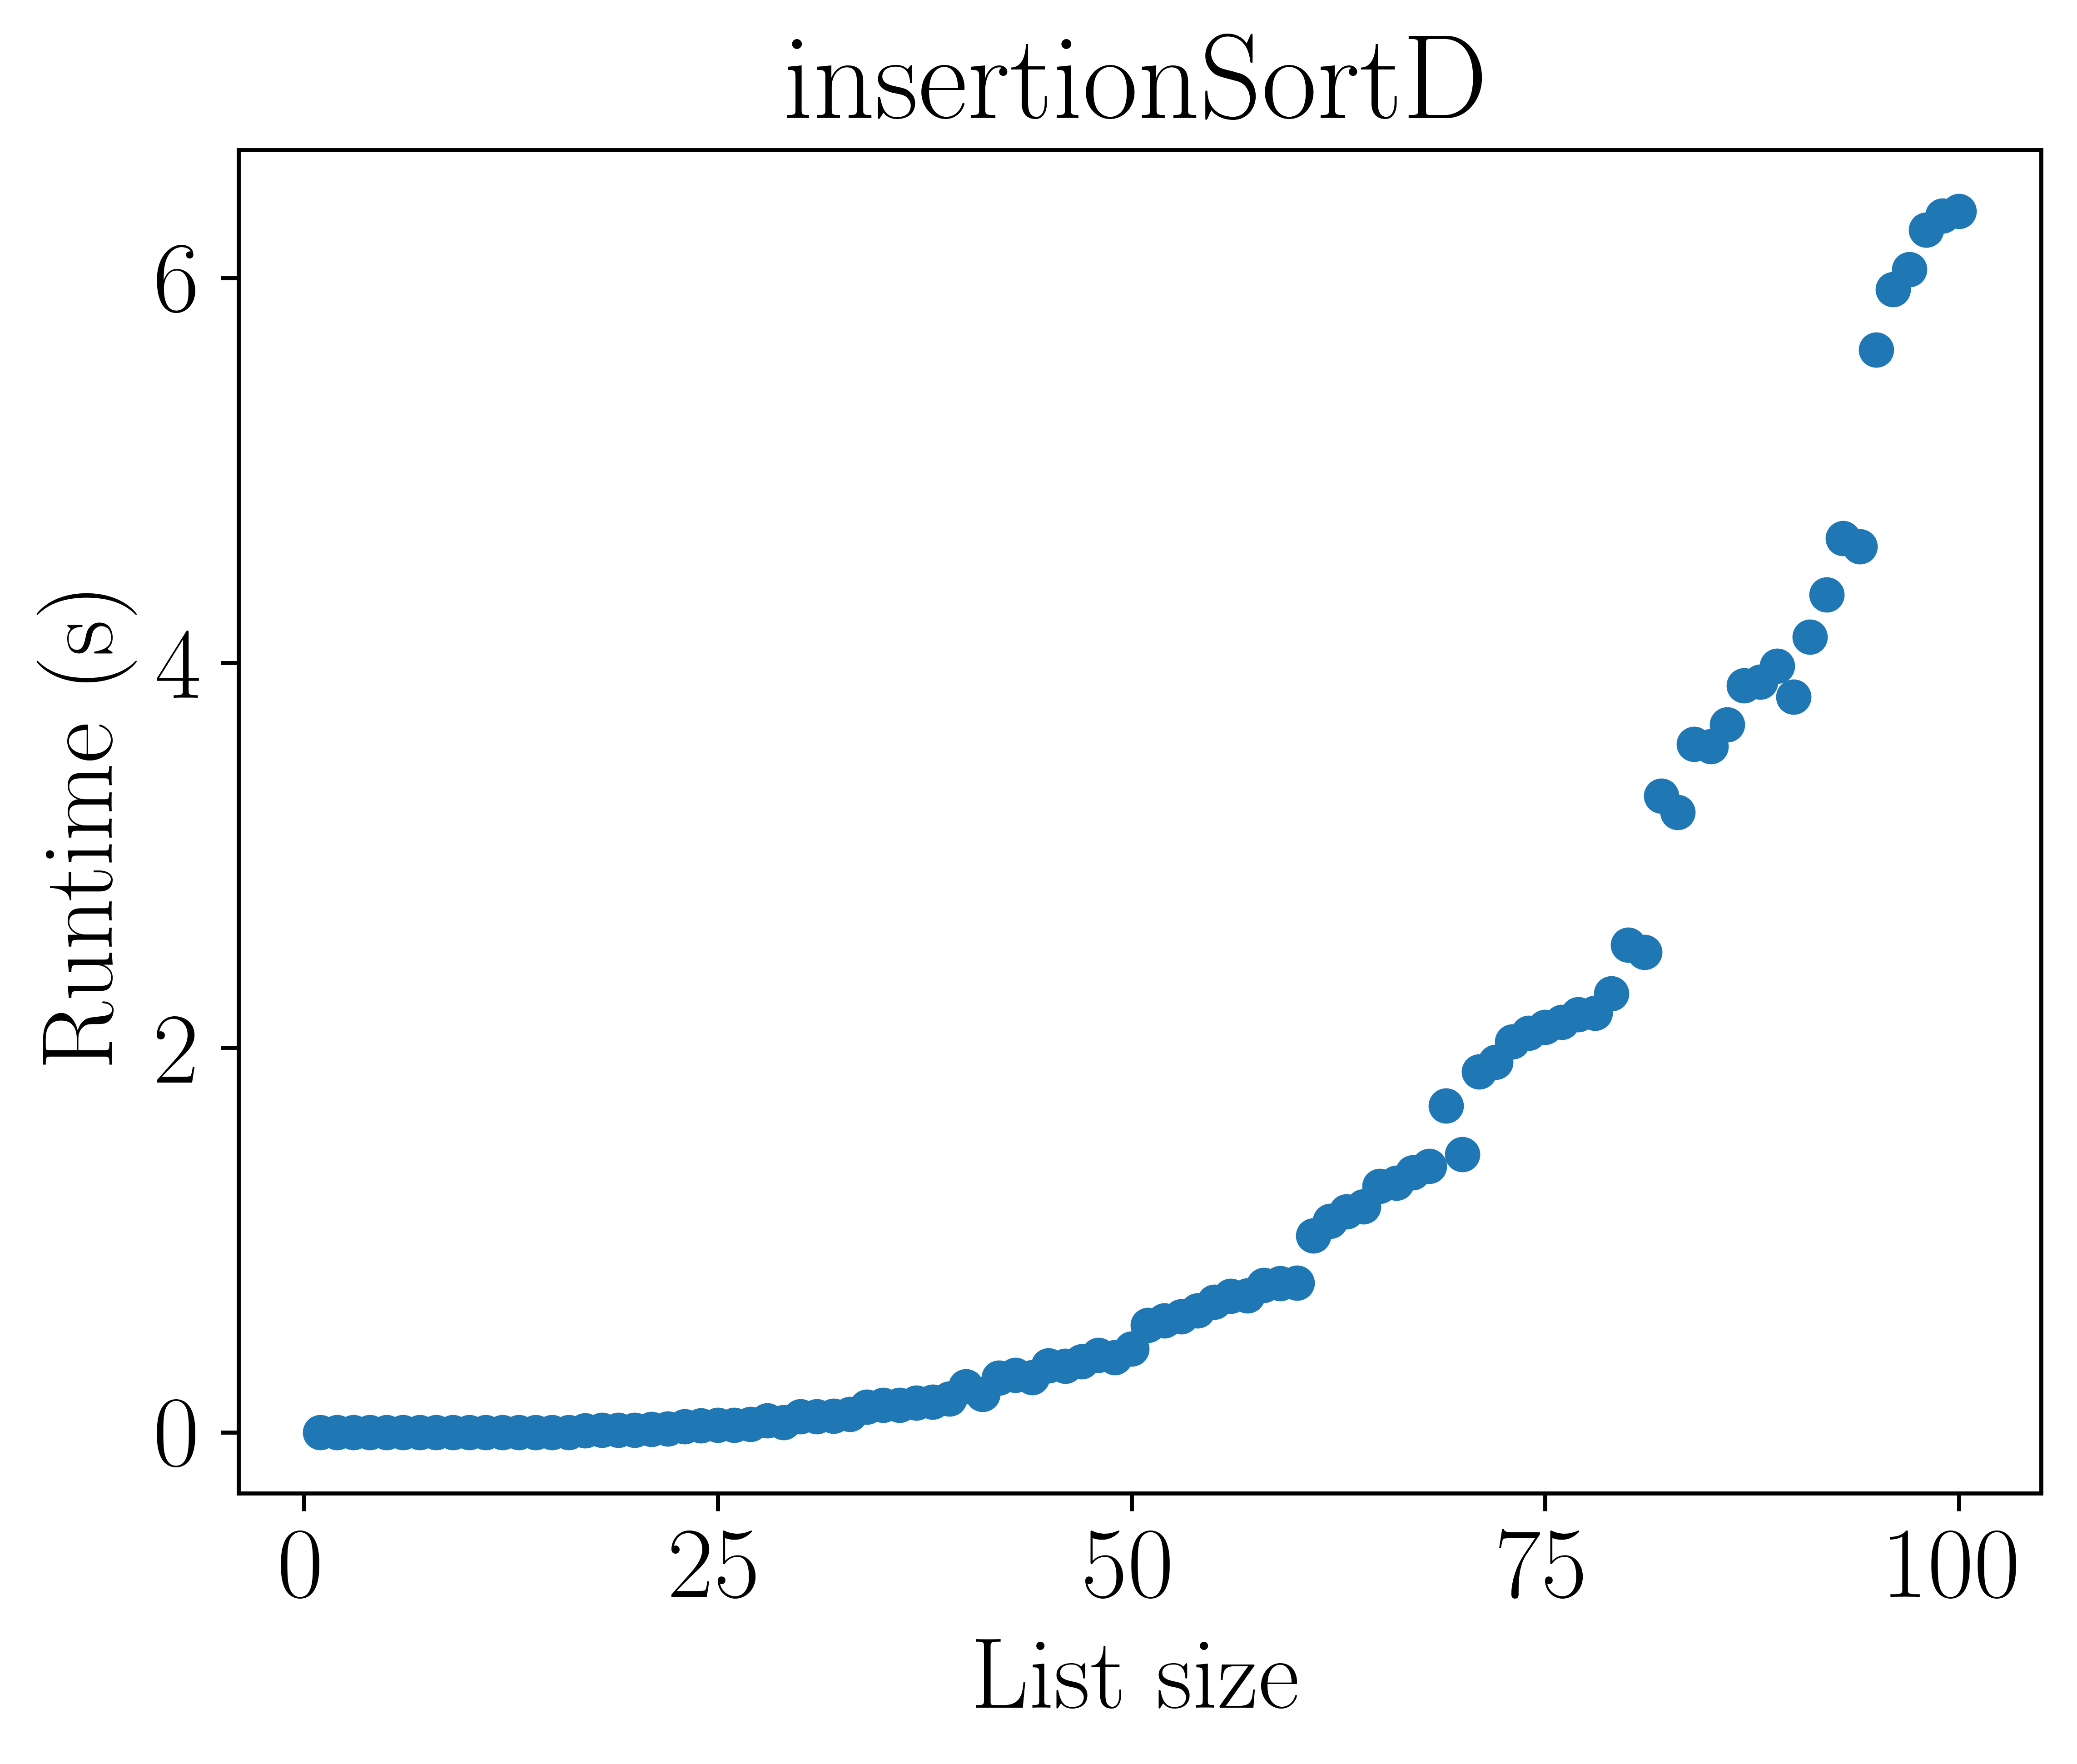
\includegraphics[width=0.55\textwidth]{Figs/insertionSortD_runtime.png}
  \caption{The runtime of
    \cdc{insertionSortD}.}\label{fig:insertionSortD_runtime}
\end{figure}

Although our translation provides a convenient way to compute demands, a
question remains about how it performs relative to hand-written demand
functions. To test this, we ran \cdc{insertionSortD} on lists of the form
\cdc{[n, n-1 .. 1]} with sizes ranging from \(1\) to \(100\), demanding the
full result each time (\cref{fig:insertionSortD_runtime}). All tests were
performed on an AMD Ryzen 3900X running Linux 6.12.58 using the built-in timing
functionality of KiCS2 version 3.5.0

Asymptotically, \cdc{insertionSortD} appears to run in \(O(n^3)\) time: a
cubic interpolation estimates it well. This asymptotic bound is shared by the
hand-written version, which, in the worst case, must call the pure
\cdc{insertionSort} function \(n\) times.  However, the constants are much
worse: \cdc{insertionSortD} takes more than \(6\) seconds on a
\(100\)-element list, while the hand-written version is fast enough that its
runtime cannot be reliably measured.
